% chapter4.tex (Chapter 4 of the thesis)

\chapter{Findings and Research Implications}\label{ch:chapter4}
In this chapter, I will be presenting my findings as an instructive manual for composers and performers interested in using the techniques.
Because my folio of works has some degree of overlap in usage of techniques, this chapter will deal with each technique, rather than be a review of findings from each piece singularly.
Where relevant, I will include my findings from working with performers.

Due to the limited number of permutations of these techniques, the Dick model of categorization is unnecessary, as space is not at a premium.\autocite{dickOtherFlute1989} 
It will also take into account how common the technique is, as well as notational challenges.

\subsection{Notation}
If the composer wishes to use a technique once off, or in sparing amounts, the technique can be shown with plain English text explaining what is desired of the player.\autocite[494]{gouldBars2011}
For all other cases where a technique is used multiple times, composers must include the technique in the frontmatter of the work that it is used in.\autocite[494]{gouldBars2011}
If a technique uses a new symbol or notehead, this should be reflected in the frontmatter.
Where possible, composers should retain the same clef for both fingered and sounding pitches.\autocite[422]{gouldBars2011}
Composers would do well to include a description of the desired sound, and method of production; example frontmatter is provided for each of the techniques, \hyperref[sec:subharmonicFrontmatter]{subharmonics}, \hyperref[sec:multiphonicFrontmatter]{multiphonics}, and \hyperref[sec:halfHarmonicFrontmatter]{half-harmonics}. 


\section{Subharmonics}\label{sec:subharmonics}
Subharmonics are a difficult technique that lend themselves to solo works, or works where they can be brought to the forefront.
They produce a sound lower than the fundamental through precise control of torsional oscillation, which usually produces the sound of an amateur string player's heavy handed, slow bowing. 
The timbre of overpressure can vary, but is identifiably pitched, and typically is somewhat nasal.
They are notably different to overpressure, but bleed over into non-pitched overpressure is common.
This, plus the difficulty in their execution, makes them unsuitable for melodic content.

Several different intervals are available as subharmonics, and a myriad of factors feed into which are easily replicable, but as a rule, octaves come most easily, with minor seconds, major sevenths, and perfect fifths coming after that.
Composers should be aware that producing the specific pitch is not \emph{necessarily} guaranteed.
Subharmonics are unable to be performed \emph{laissez vibrer}, as the pitch returns to the fundamental as soon as the bow is no longer in contact with the string.\autocite[]{appleseedFeedbackExploratorySession2019}
Due to the pressure needed, subharmonics are most comfortable at at least \emph{mezzo-forte}, although quieter subharmonics are possible. 
Sympathetic resonances from the other strings are common at higher volumes.
Playing on the two inner strings is slightly harder due to the angle of attack being restricted to not inadvertently play double-stopped notes.\autocite[99]{welbanksFoundationsModernCello}



Composers looking to use this technique should be aware that it is not a standard technique, and instrumentalists will need copious amounts of practice and guidance in order to fully and reliably realise this technique.

\subsection{Considerations for players}
Rope core strings produce more harmonics, but are more difficult to produce subharmonics with.
Strings with a single or nylon core make the technique easier, due to their low tension.\autocite[99]{welbanksFoundationsModernCello}
Players may find that subharmonics are easier on older strings, and they may also find that adding twists to the string may also help, or hinder the production of subharmonics, as shown in \autoref{tab:twistTable}.\autocite[]{kimuraHowProduceSubharmonics1999}


Botting notes that experimentations with octavic subharmonics yielded a pitch slightly flatter than an octave. He states: \begin{quotation}
  I developed a left hand finger technique whereby I rotate my hand slightly clockwise, pivoting on the finger stopping the string, which has the effect of sharpening the subharmonic enough to be more in tune with the fundamental.\autocite[111]{bottingDevelopingPersonalVocabulary2019}
\end{quotation}

To `find' the subharmonic, an excellent method to practice is to play \emph{sul ponticello} at a \emph{forte} dynamic on an open string, and then move towards the fingerboard, keeping the pressure but slowing the bowing speed down.
Subharmonics are easier to find at nodal points, particularly the 6th node (closest to the bridge).\autocite[]{appleseedFeedbackSightreadingSession2019}

Bow pressure should be totally consistent throughout the bowing stroke; rather than the tapered start and finish of \emph{normale}, players should imagine a more binary stop and start, beginning and ending on the string.
The bow hair should remain flat throughout the stroke, in order to to exert the maximum amount of pressure.\autocite[]{kimuraHowProduceSubharmonics1999}
Different bow positions on the string can make different subharmonics speak more easily.\autocite[]{kimuraHowProduceSubharmonics1999}

\subsubsection{Instrument specific considerations for subharmonics}
Subharmonics are easier to produce on the contrabass with a lighter bow, preferably a cello bow, or alternatively a French style bow.\autocite[]{longSubharmonics2019}
Conversely, violin and violas may benefit from the use of a heavier bow.\autocite[]{appleseedFeedbackSightreadingSession2019}
The tension of the string appears to impact the feasibility enormously; 13 inch violas may have more success producing subharmonics on the A string than 18 inch violas.\autocite[]{appleseedFeedbackSightreadingSession2019}



\subsection{Notation of Subharmonics}\label{sec:notation-subharmonics}
% Subharmonics should be notated with a square notehead, and a small notehead (optionally in parenthesis) at the desired pitch.
Subharmonics require both a fingered pitch, and an intended resultant pitch to be conveyed to the player, as well as some form of indication that it is a subharmonic.
This can be done through a variety of ways, including technique text (i.e.\ `S.H.' as Long suggests), or using a different notehead.\autocite[]{longSubharmonics2019}

Gould suggests several practical methods of communicating resultant pitch, as a ``small [black] notehead [without a stem] in brackets directly above or after the fingered pitches'', an ossia stave with the resultant pitches above, or notated in a footnote using a cue stave.\autocite[421]{gouldBars2011}
She states ``wherever possible, retain the same clef for both fingered and sounding pitches'', though this is sometimes impractical.\autocite[422]{gouldBars2011}
% This is sometimes practical, but gives rise to the issue of indicating pitch. 
The use of a second stave is seen in \autoref{fig:Excerpt from Risset's Variants}.\autocite[It should be noted that Risset's notation omits a fingered pitch, which is not recommended.]{rissetVariants1995}
Extrapolating from the use of the circular harmonic signifying at-pitch harmonics, we can apply the same method to subharmonics, as seen in \autoref{fig:subharmonicsNotationExampleTwoStave}.
\begin{figure}
  \centering
  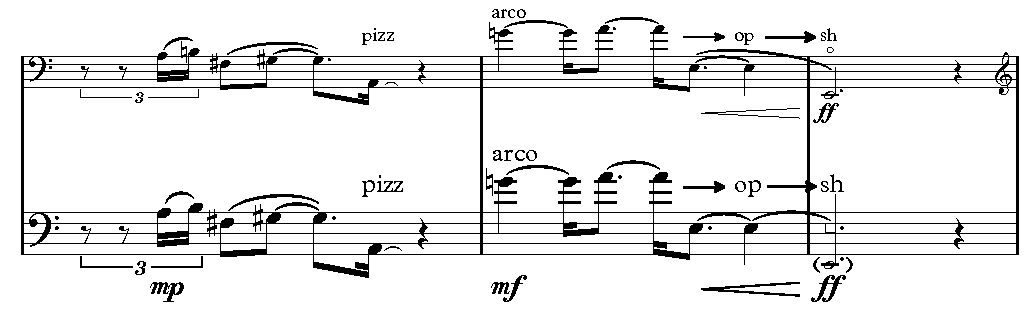
\includegraphics[width=\linewidth]{./resources/subharmonicsNotationExample.pdf}
  \caption{Excerpt from \bassPiece\space showing subharmonics notation.}\label{fig:subharmonicsNotationExampleTwoStave}
\end{figure}

% TODO: Example of Subharmonics --- https://trello.com/c/bc3sNJTL/32-example-of-subharmonics


\subsubsection{Subharmonic Frontmatter}\label{sec:subharmonicFrontmatter}

\subsection{Works featuring subharmonics }\label{sec:subharmonicsLiterature}

\begin{itemize}
    \item Mari Kimura --- ALT in three movements for solo violin (1992)
    \item --- Gemini for solo violin (1993)
    \item --- 6 Caprices for subharmonics for solo violin (1997) 
    \item --- JanMaricana (for subharmonics) for solo violin (2016)
    \item Joshua Burel --- Sonata No. 2 for violin and piano `Subharmonics' (2011)
    \item Jean-Claude Risset --- Variants (1995)
    \item Robert Rowe --- Submarine (1996)
\end{itemize}

\section{Multiphonics}\label{sec:multiphonics}

Multiphonics are fragile, and require much practice to execute reliably.
Despite this, they can be used to achieve harmonies that are not otherwise achieveable through double-stopping, and lend themselves well to drawn out or slow passages of music. 
Multiphonics' exact pitching makes them ideal for music that uses ratios, microtones, or tone rows. 
Multiphonics are easier to achieve on larger instruments, due to the need for precise ratio-based fingering to achieve the resonance of multiple partials.

The open string (or first partial) can be activated as part of a multiphonic.\autocite[161]{welbanksFoundationsModernCello}
The second partial (octave harmonic) is \emph{never} produced in a multiphonic


\subsubsection{Considerations for players}
Multiphonics should be played closer to the bridge than one would normally play them.
Overly high and low bow pressure can limit the lower partial content of resultant multiphonics.
Faster bow speed favours higher partials over lower partials, and similarly, slower bow speed favours lower partials over higher.
Moving the contact point closer to the bridge yields more noise content and favours lower partials, until the contact point is very close to the bridge, where it produces a clearer sound and favours higher partials over lower partials.\autocite[http://www.cellomap.com/index/the-string/multiphonics-and-other-multiple-sounds.html]{fallowfieldCelloMap}
Multiphonics containing higher partials require a lighter and faster bow stroke, closer to the bridge than multiphonics that have lower ranges of partials.\autocite[165]{welbanksFoundationsModernCello}

To first find a multiphonic, Welbanks and Fallowfield both recommend playing the harmonics individually.\autocite[167]{welbanksFoundationsModernCello}
Then play the harmonic with the highest resultant pitch. 
Use a slower bow stroke with higher pressure and closer to the bridge, and slightly lighter finger pressure.


\subsubsection{Instrument specific considerations for multiphonics}
Multiphonics are easier on large instruments, as more precise pitching is possible with the longer strings.
Composers should be aware that of the pair, the multiphonic node closer to the bridge can be harder to produce because of this fact.
`Artificial' multiphonics are possible, although much more difficult.\autocite[772]{guettlerBowedstringMultiphonicsAnalyzed2012}

\subsection{Notation of Multiphonics}\label{sec:notation-multiphonics}
Much has been written about multiphonics, and they are a well established technique in woodwind writing.
The notation between them differs, though; precise fingering charts above resultant pitches do not translate precisely into string writing.\footnote{The relation between string and woodwind multiphonics is discussed more in-depth \hyperref[sec:multiphonicsWoodwind]{in chapter 2.}}
Fallowfield states: \begin{quotation}
    To notate ‘pure’ multiphonics accurately in a score, however, it is necessary to indicate both the left-hand finger position and the pitch content. 
    The left-hand finger touches the string above the node of the highest harmonic that contributes to the multiphonic, so the finger position is always that of the highest harmonic in the group. 
    I suggest notating finger position with the rhombus that is usually used for harmonic finger pressure. 
    The pitch of the contributing harmonics could be notated in brackets or on a separate stave.
    It is necessary to indicate which string the multiphonic should be played on and helpful to use the indication ‘M’ for multiphonic.\autocite[http://www.cellomap.com/index/the-string/multiphonics-and-other-multiple-sounds.html]{fallowfieldCelloMap}
\end{quotation}
Below, I have notated the permutations of what Fallowfield has described, and will let the reader draw their own conclusion as to which is most appropriate.
Her example omits the necessary string, but Gould suggests several different options; the inclusion of the corresponding string number (i.e.\ `I', `IV'), the usage of Italian (i.e.\ `sul E', `sul G'), or by notating the fundamental on the stave, using ``a small bracketed black notehead (regardless of duration) for the open string and for the first note only of a tied harmonic.''\autocite[418]{gouldBars2011}
In \autoref{fig:multiphonicNotationCent}, we see the specific cents tuning for the fingered note, contrasted with \autoref{fig:multiphonicNotationQuarter}, which uses quarter tones to convey the relevant pitching data, both with a \emph{suono reale} stave indicating the sounding pitch above.

\begin{figure}
  \centering
  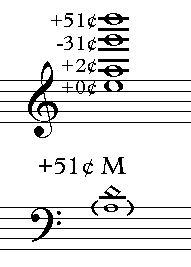
\includegraphics{./resources/multiphonicNotationCent.pdf}
  \caption{Multiphonic notation with cents}\label{fig:multiphonicNotationCent}
\end{figure}

\begin{figure}
  \centering
  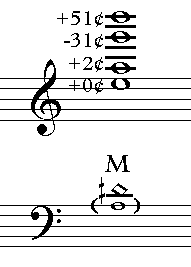
\includegraphics{./resources/multiphonicNotationQuarter.pdf}
  \caption{Multiphonic notation with quarter tones}\label{fig:multiphonicNotationQuarter}
\end{figure}
While \autoref{fig:multiphonicNotationCent} is more precise, the horizontal space usage is greater than that of \autoref{fig:multiphonicNotationQuarter}; if using text to specify which string to use, it may quickly become cumbersome to read.


Gould's advice for resultant pitch for harmonics, which has been applied to subharmonics can also be applied to multiphonics as evidenced in \autoref{fig:multiphonicNotationOneLine}
The ossia staff, or \emph{suono reale} if necessary for the entirety of the work\footnote{\emph{suono reale} should be full sized, while ossia staves are 3/4 sized.}, can have the multiphonics notated as a rhythm, as seen in \autoref{fig:multiphonicNotationOssia}.

\begin{figure}
  \centering
  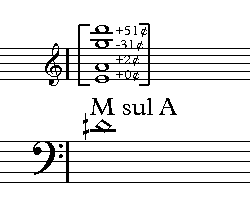
\includegraphics{./resources/multiphonicNotationOssia.pdf}
  \caption{Multiphonic notation using an ossia line}\label{fig:multiphonicNotationOssia}
\end{figure}

\begin{figure}
  \centering
  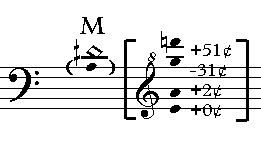
\includegraphics{./resources/multiphonicNotationOneLine.pdf}
  \caption{Multiphonic notation on one line}\label{fig:multiphonicNotationOneLine}
\end{figure}

Further simplifications can be made if there is no clef change, making it possible to omit the `M' technique text denoting it as a multiphonic.

\begin{figure}
  \centering
  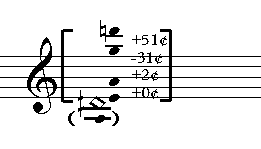
\includegraphics{./resources/multiphonicNotationOneLineClef.pdf}
  \caption{Multiphonic notation in one clef}\label{fig:multiphonicNotationOneLineClef}
\end{figure}

There are several ways of notating the same (or similar) information, and due to the cumbersome nature of multiphonics, there is often a deficit of either vertical or horizontal space.
However, with the flexibility of each element, there is surely be a method of notating multiphonics idiomatically that can be implemented in every score that makes use of them.

\subsubsection{Multiphonic Frontmatter}\label{sec:multiphonicFrontmatter}
\begin{quotation}
  
  Multiphonics are achieved through clusters of close harmonic nodes, and by playing a harmonic close to the highest partial.
  Note that not all of these pitches will actually sound in practice.
  
  Multiphonics are notated as a harmonic position, with an `M' above the note to be fingered.
  Where the string used is ambiguous, it is notated below the sounding pitch as a small, bracketed notehead.

  Precise tuning is given in cents, and unless otherwise notated, is intended for the first note that the multiphonic is attached to.\footnote{100 cents is equal to a semitone. Therefore, +51c is roughly equal to half a semitone sharp. Cents have been used due to their precision compared to more granular accidentals such as the quartertone sharp.}
  The theoretical sounding pitches are given in a bracketed staff above the main stave.
  % Above the sounding pitches, the sounding partials are given (i.e. M IV [4th + 13th + 9th + 15th + 5th]).

  The bow should exert slightly more pressure than usual and should be drawn with a consistent speed which should be slower than for harmonics.
  The location of the bow can encourage or discourage upper or lower partials, and experimentation should be done during the practice of this work to achieve the pitches desired.
\end{quotation}


\subsection{Works featuring multiphonics}\label{sec:multiphonicsLiterature}
% TODO: Find multiphonic works --- https://trello.com/c/o75LaLo8/13-find-multiphonic-works

\begin{itemize}
    \item Mari Kimura --- 6 Caprices for subharmonics for solo violin (1997) 
    \item Andrew Greenwald --- On Structure (2a) --- for clarinet, violin, and cello (2010)
    \item Stefano Scodanibbio --- composed e/statico (1980)
    \item Håkon Thelin --- oibbinadocS (2004)
    \item --- Glasperlenspiel (2010)
    \item Michael Liebman --- Sonata for double bass, movement 2: Legato sonore (2001)
    \item Kaija Saariaho --- Lichtbogen (1986)
    \item Kimmo Hakola --- Thrust, Rubato (1989, rev. 1991) 
    \item Eivind Buene --- `Blacklight' (2019)
    \item Fernando Grillo --- `Fluvine' (1974)
% Brian Ferneyhough Trittico Per G.S
% Iannis Xenakis' \emph{Theraps} for solo contrabass is \lipsum[1].\autocite[]{}
% Barry Guy Statements II
\end{itemize}

\section{Half-harmonics}\label{sec:half-harmonics}
Half-harmonics are produced via left-hand finger pressure that is halfway between that of a harmonic and a \emph{normale} sound produced when the string is pressed to the fingerboard.
The pitch content is sharpened slightly, and the overtone content is relatively weak.\autocite[113]{welbanksFoundationsModernCello}
Half-harmonic stops are not limited to the nodes and hence the natural harmonics, but may be executed on all fingerboard positions, as well as executed as `artificial' harmonics.\autocite[127]{dimpkerExtendedNotationDepiction2012} 
Half-harmonics are what many would interpret as notes that `fail to speak'.

\subsubsection{Considerations for players}
Half-harmonics are pitched slightly sharp, and so should be fingered accordingly flat to compensate for this.\autocite[113]{welbanksFoundationsModernCello}

\subsection{Notation of Half-harmonics}\label{sec:notation-half-harmonics}
Half-harmonics can be notated in one of several ways (see \autoref{fig:halfHarmonicNotationExamples} for examples of both the crotchet and semibreve notation of each), but regardless of the chosen symbol, should be included and described in the performance notes.


\begin{figure}
    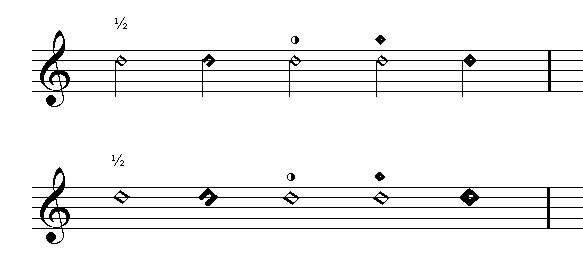
\includegraphics[width=\linewidth]{./resources/halfHarmonicNotationExamples.pdf}
    \caption{Half-harmonic notation examples}\label{fig:halfHarmonicNotationExamples}
\end{figure}

  
The simplest method, using text rather than a graphic may produce good results, as seen in \autoref{fig:textSymbolNotation}.
No scores appear to use this method, despite it being the only example able to convey more precise ratios of finger pressure as Fallowfield states is possible.\autocite[http://www.cellomap.com/index/the-string/multiphonics-and-other-multiple-sounds/other-multiple-sounds.html]{fallowfieldCelloMap}

\begin{figure}
  % \includegraphics[width=\linewidth]{./resources/circleExample.pdf}
  \includegraphics[page=1,width=\textwidth]{resources/halfHarmonicsSingleExamples.pdf}
  \caption{Half-harmonic displayed with text}\label{fig:textSymbolNotation}
\end{figure}

The second and last of the examples in \autoref{fig:halfHarmonicNotationExamples} do not have discrete noteheads for crotchets and minims like regular diamond noteheads.
As such, if there is rhythmic ambiguity, rhythms should be clarified above the stave as normal.
The second example, as seen in Sciarrino's \emph{Six Capricci for Violin} (\autoref{fig:sciarrinoExcerpt}) shows the ambiguity of this.
The `slant' of the regular harmonic notehead is opposite to the unfinished diamond, going from up to down, helping distinguish it.

The third example unfortunately is not without issues, either; (\emph{normale}) harmonics denoted with a circle are exclusively for the resultant pitch.\autocite[419]{gouldBars2011} 
While half-harmonics do produce the notated pitch, rapid transitions between half-harmonics and \emph{normale} harmonics using half-filled circles may cause confusion due to the translation between a symbol that denotes pressure needed and a resultant harmonic respectively, as illustrated in \autoref{fig:circleExample}, which is the notation used for half-depressed valves on brass instruments.\autocite[85]{cherryExtendedTechniquesTrumpet2009}
This is compounded by the circle notation's inability to handle harmonics that fall well outside the range of the staff (i.e.\ major 3rd and minor 3rd harmonics), resulting in a need for at least two types of notation; circular half-harmonics, and diamond noteheads for problematic \emph{normale} harmonics.

\begin{figure}
    % \includegraphics[width=\linewidth]{./resources/circleExample.pdf}
    \includegraphics[page=3,width=\textwidth]{resources/halfHarmonicsSingleExamples.pdf}
    \caption{Half-harmonic circular notation}\label{fig:circleExample}
  \end{figure}

The fourth example of notation displayed in \autoref{fig:diamondSymbolNotation} is a non-standard symbol, and also suffers the same issues that plague the previous example.

\begin{figure}
  % \includegraphics[width=\linewidth]{./resources/circleExample.pdf}
  \includegraphics[page=4,width=\textwidth]{resources/halfHarmonicsSingleExamples.pdf}
  \caption{Half-harmonic diamond symbol notation}\label{fig:diamondSymbolNotation}
\end{figure}


Compare this with \autoref{fig:halfFilledNotation} and \autoref{fig:halfEmptyNotation}, which is an example of Sciarrino's half-empty notation as seen in \autoref{fig:sciarrinoExcerpt}.

\begin{figure}
  % \includegraphics[width=\linewidth]{./resources/circleExample.pdf}
  \includegraphics[page=5,width=\textwidth]{resources/halfHarmonicsSingleExamples.pdf}
  \caption{Half-harmonic half-filled notehead}\label{fig:halfFilledNotation}
\end{figure}


\begin{figure}
  % \includegraphics[width=\linewidth]{./resources/circleExample.pdf}
  \includegraphics[page=2,width=\textwidth]{resources/halfHarmonicsSingleExamples.pdf}
  \caption{Half-harmonic half-empty notehead}\label{fig:halfEmptyNotation}
\end{figure}


  % \begin{figure}
  %   \includegraphics[width=\linewidth]{./resources/diamondExample.pdf}
  %   \caption{Half-harmonic diamond notation}\label{fig:diamondExample}
  % \end{figure}

  % \begin{figure}
  %   \includegraphics[width=\linewidth]{./resources/diamondExample2.pdf}
  %   \caption{Half-harmonic diamond notation with circle notation}\label{fig:diamondExample2}
  % \end{figure}

% Further simplications on the stave are possible as evidenced in \autoref{fig:halfHarmonicNotationExample3} by denoting the string using text, or if sequential, lines.

% \begin{figure}
%     \includegraphics[width=\linewidth]{./resources/halfHarmonicNotationExample3.pdf}
%     \caption{Half-harmonic diamond notation with string specification}\label{fig:halfHarmonicNotationExample3}
%   \end{figure}



It should be noted that the half-filled notehead as depicted in Gould and \autoref{fig:halfFilledNotation}, nor the Sciarrino style half-empty notehead as seen \autoref{fig:halfEmptyNotation} are not available in modern versions of Sibelius or Dorico as of the time of writing.\autocite[424]{gouldBars2011}
The flagship Standard Music Layout Font (SMuFL), Bravura, includes the half-harmonic circle as depicted in \autoref{fig:circleExample}, but is only available on Dorico and the Sibelius port of Bravura, Norfolk.\autocite[]{w3ccommitteeStandardMusicFont2019}

\subsubsection{Half-harmonic Frontmatter}\label{sec:halfHarmonicFrontmatter}
Half-harmonics are produced by applying left hand finger pressure halfway between that required to create a harmonic, and a \emph{normale} sound. 
The sound that is produced should be a mixture of the stopped string pitch, the harmonic pitch, and a resistant, slightly noisy quality.
They are notated in the score as a half-filled diamond notehead.
\subsection{Works featuring half-harmonics}\label{sec:half-harmonicsLiterature}

\begin{itemize}
    \item Robert Rowe --- Flood Gate (1989)
    \item Salvatore Sciarriono --- 6 Capricci for violin (no. 5) (1976) 
    \item Helmut Lachenmann, Gran Torso
    \item Trevor Bača --- Al-Kitab Al-Khamr (2015)
    \item Claudio Pompili --- Scherzo Alla Francescana (1990, revised 1994)
    \item Mary Bellamy --- Transference (?)
    \item Sam Park --- The Colour of Light (2010)
    \item Jack Symmonds --- Hell Is Murky (2018)
    \item Mark Applebaum --- The Plate of Transition Nourishes the Chameleon Appetite (1992, revised 1994)
    \item Henrik Deneren --- seals II (2014--15)
    \item Ramteen Sazegari --- Slate Representative (2015)
\end{itemize}

\section{Reflection}




\lipsum[4]